\section{Optimering}
Nu er systemet sat sammen og skal til at optimeres og korrigeres til en ønsket respons. I første omgang er denne ønskede respons så flad så muligt ned til omkring 50Hz. For at se hvad udgangspunktet for højtaleren med enhederne indsat i det modificerede kabinet med det valgte delfilter laves at frekvenssweep (1 meter afstand) for at se hvordan frekvenskarakteristikken ser ud. Dette kaldes også standard konfigurationen (config 1).  
Udgangspunktet for venstre side af højtaleren kan ses i \autoref*{fig:Standard-udgangspunkt}

\begin{figure}[H] 
	\center
	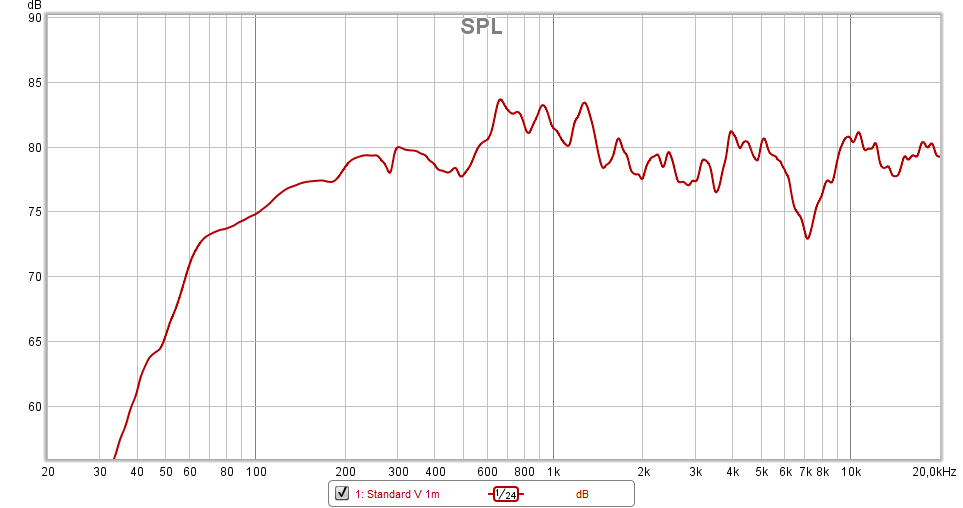
\includegraphics[width=1\linewidth]{figur/Standard-udgangspunkt}\quad
	\caption{Frekvenskarakteristik venstre side udgangspunkt}
	\label{fig:Standard-udgangspunkt}
\end{figure}

Det kan i \autoref{fig:Standard-udgangspunkt} ses at den akustisk kortslutning forsvundet efter enhederne er kommet i kabinet. Det ses også at for generelt at gøre responsen flad kræver det at frekvenserne for basenheden under 400-500Hz forstærkes/boostes og især ved omkring 60Hz, hvis responsen skal være flad ned til omkring 50Hz. Derudover skal frekvenserne for diskanten generalt også hæves en smule, så det udligner det amplitude peak mellem 600hz og 1200 Hz. 

Derfor laves der i på MiniDSP'en et parametrisk EQ filter (IIR) til at booste bassen hos basenhederne og ligeledes et parametrisk EQ filter (IIR) til at løfte diskanterne lidt op. Dette kan ses i BLA BLA BLA

\subsection{Korrektion af enheder}



\subsection{EQ af med FIR filtre}
\subsubsection{Rock}
\subsubsection{Jazz}
